\chapter{Metodología}
\label{chap:methodology}

En este capítulo se describirá la metodología propuesta, formulada a partir de las conclusiones extraídas del capítulo \ref{chap:stateofart}. Posteriormente, se realizará una revisión de dicha metodología con la experiencia obtenida tras completar el desarrollo del juego, el cual se detalla en el capítulo \ref{chap:development}.

A continuación se recapitulan los riesgos y problemas más comunes en el desarrollo de videojuegos:

\begin{enumerate}
    \item \textbf{Alcance del proyecto y \textit{feature creep}}, la adición descontrolada de contenido por planificación pobre.
    \item \textbf{Integración de recursos multimedia} como arte o sonido.
    \item \textbf{Convivencia del proceso creativo con el de ingeniería}, tanto de las distintas disciplinas asociadas como de la construcción del propio videojuego.
    \item \textbf{Búsqueda del \textit{fun factor}}.
    \item Gestión de proyectos con plantillas de empleados grandes y diversas.
    \item \textbf{Satisfacción del público objetivo del juego}, calibrar la experiencia para que esté al nivel de dificultad esperado.
    \item \textbf{Uso de crunch}, o agotar el presupuesto del proyecto.
\end{enumerate}

Para diseñar la metodología que se expone a continuación se buscó abarcar todos los puntos de la lista anterior con la excepción del punto 5. Esto se debe a que este es un proyecto individual en el que una sola persona que asume todos los roles.

El desarrollo contará con 4 fases: \textbf{preproducción, producción, postproducción} y \textbf{despliegue}.

\section{Preproducción}

\begin{figure}[H]
    \centering
    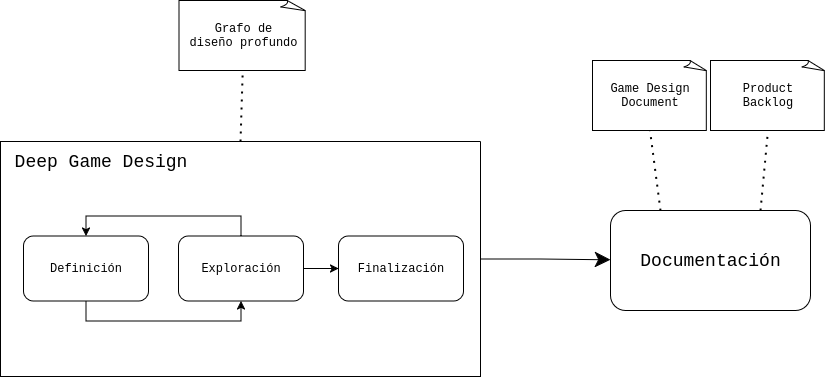
\includegraphics[scale=0.50]{img/preproduction.drawio.png}
    \caption[Diagrama de preproducción]{Diagrama del proceso de preproducción.}
    \label{fig:preproduction}
\end{figure}

La preproducción comienza aplicando \textbf{Deep Game Design} \cite{deepdesign}. Se experimentará con prototipos rápidos y baratos las ideas de diseño sobre las que se cimentará el juego. Se plantearán y verificarán las distintas restricciones (es decir, las mecánicas y reglas del juego) y los diferentes puzles (desafíos) que se le plantearán al jugador. En esta fase se producirá el \textit{diagrama de diseño profundo}, con sus métricas de profundidad, complejidad y elegancia. Una vez finalizada esta fase, se tendrá una comprensión profunda de las mecánicas principales alrededor de las que se construirá el juego.

Con este conocimiento adquirido se pasará a desarrollar una primera iteración del \textit{Game Design Document} (GDD), donde se desarrollará el \textit{pitch} (concepto) del juego, su contexto, narrativa, mecánicas principales, estilo artístico, estructura general del juego, etc. Este documento podrá ser modificado en etapas posteriores.

A continuación se redactará el \textit{product backlog}. Esto es un artefacto de SCRUM, ya que en producción se trabajará con una versión adaptada de esta metodología. Se trata de una lista ordenada de requisitos del proyecto, normalmente en forma de historias de usuario.

Las \textbf{historias de usuario} son requisitos formalizados desde la perspectiva del usuario. Suelen tener la misma estructura:\\ 


\centerline{\textit{Como [tipo de usuario] quiero hacer [actividad] para [objetivo]}}

Por ejemplo: \textit{''como usuario, quiero poder revisar la foto que acabo de hacer con la cámara de mi móvil para comprobar si he salido bien''}. Este formato es ideal para expresar requisitos funcionales. Se realiza desde la perspectiva del usuario expresando una necesidad suya, y no una solución de implementación concreta. En este proyecto se emplearía para cuestiones como funciones de guardado, de accesibilidad o de ajustes de usuario. Sin embargo, como se ha comentado anteriormente, no se puede expresar el núcleo jugable del juego, su estética o su \textit{fun factor} con la estructura de una historia de usuario. Para ello se propone el siguiente artefacto: \textbf{historia de juego}.

Las historias de juego son una formalización de las ideas plasmadas en el \textit{GDD}. Su objetivo es representar los requisitos emocionales y abstractos del proyecto y poder añadirlos al \textit{product backlog}. Siguen la siguiente estructura:\\

\centerline{\textit{El [actividad/elemento] es [adjetivo]}}

Por ejemplo, \textit{es divertido rebotar en los enemigos}, \textit{es divertido recolectar monedas}, \textit{el cansancio del personaje transmite la dureza de subir una montaña}, o \textit{los entornos transmiten nostalgia}. Las historias de juego son un artefacto \textbf{exclusivamente representativo} de los requisitos emocionales del juego dentro del product backlog, siendo responsabilidad del \textit{GDD} explicarlos y contextualizarlos. Se propone hacer esto así para tenerlos como elementos operables durante los \textit{sprints} de producción y poder visualizarlos en los \textit{tableros kanban} que se realizarán en la misma.

Por último, se realizará una estimación del proyecto con un presupuesto en forma de horas efectivas de trabajo. El desarrollo completo hasta la salida del juego no deberá sobrepasar este número.

\section{Producción}

\begin{figure}[H]
    \centering
    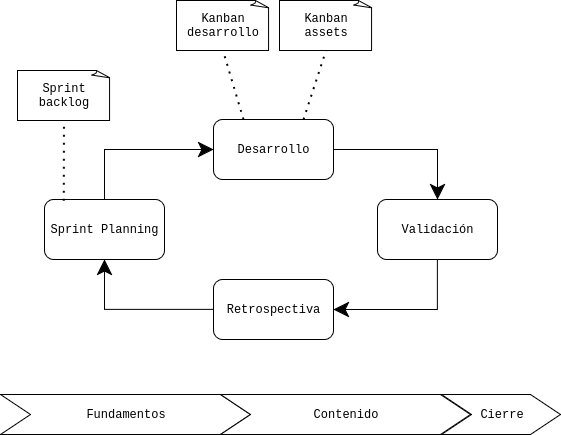
\includegraphics[scale=0.50]{img/production.drawio.png}
    \caption[Diagrama de producción]{Diagrama del proceso de producción.}
    \label{fig:production}
\end{figure}


Para la producción se usará una versión adaptada de SCRUM. Estará dividida en \textit{sprints} de alrededor de 20 horas de trabajo efectivo. Los sprints son iteraciones del proyecto con un tiempo fijo. Tienen la siguiente estructura:

\begin{itemize}
    \item \textbf{\textit{Sprint planning}}: Se revisa el product backlog, se escogen las historias de usuario que se desarrollarán en ese sprint y se derivan tareas relacionadas con estas al \textit{sprint backlog}. Para cada tarea se realiza una estimación en horas para su compleción y qué \textit{assets} se requieren.
    \item \textbf{Desarrollo}: Se hace uso de un \textit{tablero kanban} para gestionar el estado de las diferentes tareas, el cual puedes ser diseño, implementación, validación, test, finalizado y descartado. Se tiene otro tablero kanban para llevar la cuenta y el progreso de la producción de los distintos assets. En este punto se desarrollan los test automáticos asociados 
    \item \textbf{Validación}: Una vez finalizado el grueso del sprint, se realiza una sesión íntegra del producto resultante. Durante esta se realizan anotaciones sobre la experiencia percibida, las sensaciones, qué elementos funcionan a nivel emocional y cuáles no. Si se detecta algún problema en esa línea, se anotará en el product backlog en forma de \textbf{observación de test}. Esta es un tipo de entrada al mismo nivel que las historias de usuario o juego. En él se describe el problema detectado en el juego, para el cual deberá diseñarse una solución en sprints posteriores.
    \item \textbf{Retrospectiva}: Se realiza un repaso del desempeño del sprint, redactando en un pequeño documento qué se ha hecho bien, qué se ha hecho mal, qué imprevistos han surgido y cómo se adaptará el proyecto en siguientes sprints. Por último se hace una primera aproximación sobre qué parte del product backlog se tratará en el siguiente sprint.
\end{itemize}

A su vez, los sprints de producción se encasillan en tres etapas sucesivas:

\begin{itemize}
    \item \textbf{Fundamentos} (40\% del total): En esta se desarrolla el núcleo jugable y funcional del juego. Esto abarca asuntos como el bucle principal de ejecución, el desarrollo completo del personaje principal y herramientas que faciliten la creación de contenido para el proyecto, como un constructor de mapas, plantillas para implementar enemigos, un sistema de diálogos, el sistema de cámaras, etc. Es especialmente importante verificar la calidad del núcleo jugable, ya que este a penas será modificado más adelante.
    \item \textbf{Contenido} (40\% del total): Usando las herramientas de la fase anterior, se añade contenido al juego de manera iterativa: más enemigos, más escenarios, o mecánicas concretas. Por ejemplo, si se desarrolla una zona de volcanes, se implementa una mecánica a través de la cual el personaje puede quemarse con la lava. Estas mecánicas por su naturaleza puntual, deben ser más simples y sencillas de implementar que el núcleo del juego.
    \item \textbf{Cierre} (20\% del total): Se cesa de añadir contenido nuevo con el objetivo de cerrar la experiencia con lo que ya se tiene hecho. Al final de esta fase, la producción acaba y el juego debe ser jugable de principio a fin.
\end{itemize}

Durante la fase de contenidos se producirá una versión de prueba del juego. Se empleará en una prueba con usuarios reales, con el objetivo de obtener retroalimentación sobre el juego, ver qué aspectos gustan, cuáles no y poder reaccionar con tiempo para aplicar cambios en la planificación de ser necesario.

\section{Postproducción}

\begin{figure}[H]
    \centering
    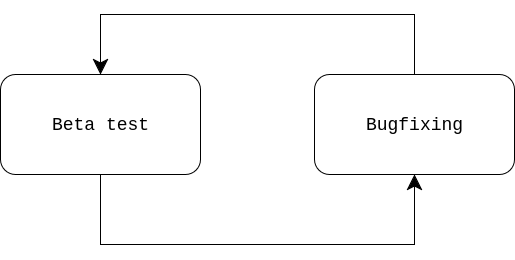
\includegraphics[scale=0.50]{img/postproduction.drawio.png}
    \caption[Diagrama de postproducción]{Diagrama del proceso de postproducción.}
    \label{fig:postproduction}
\end{figure}

Durante la postproducción se produce una fase intensiva de test para detectar y corregir bugs. Se prueba el juego por usuarios, tanto de dentro del equipo de desarrollo como fuera de él, en sesiones monitorizadas siempre que sea posible. Además de solventar bugs se realizan cambios estéticos para pulir el apartado visual. Se hace uso de un tablero kanban donde se anotan todos los bugs y problemas derivados de las sesiones de test.

\section{Despliegue}

\begin{figure}[H]
    \centering
    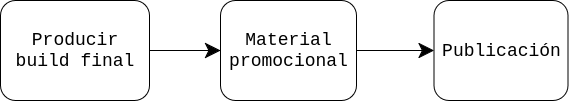
\includegraphics[scale=0.50]{img/deploy.drawio.png}
    \caption[Diagrama de despliegue]{Diagrama del proceso de despliegue.}
    \label{fig:deploy}
\end{figure}

Se compila el juego y se prepara para su publicación por el medio correspondiente (Steam, \textit{itch.io}, consolas, etc.). También se preparan materiales promocionales como un tráiler y recursos gráficos.


\section{Revisión de la metodología}

Durante el desarrollo del proyecto se realizaron las siguientes observaciones:

\begin{itemize}
    \item Deep Design es un marco de trabajo interesante, ya que aporta estructura a la búsqueda de las bases jugables e identitarias del proyecto. Sin embargo, sería más interesante usarlo en proyectos más experimentales, en lugar de un Metroidvania de corte clásico. Algunos de sus artefactos resultaron redundantes a la hora de aplicarlos a aspectos clásicos del género que ya están validados en otros juegos. Aun así, la estructura de puzles ayuda a plantear las mecánicas e interacciones.
    \item En retrospectiva, la fase de prototipado en la preproducción fue demasiado corta y el prototipo producido podría haber explorado más la identidad del proyecto. Durante el primer tercio del proyecto se sintieron dudas e inseguridades sobre la identidad del mismo.
    \item Invertir mucho tiempo en implementar requisitos funcionales en los primeros sprints hizo que se perdiera de vista la identidad del juego, lo que produjo inseguridades.
    \item Se realizó playtesting en casi todas las etapas de la producción, pero el verdaderamente valioso fue a partir del sprint 5, donde ya existían niveles que el jugador podía completar.
    \item Las iteraciones del proyecto se plantearon por bloques de funcionamiento. Es decir, en la mayoría de casos, dentro de un sprint se planteaba la implementación completa de N sistemas o funcionalidades. Esto provocó que no hubiera tiempo en los sprints para generar contenido jugable con el que hacer un playtesting valioso.
\end{itemize}

Dadas estas observaciones, \textbf{se proponen estos cambios} al proceso de desarrollo, que se aplicarían en caso de emprender un segundo proyecto:

\begin{itemize}
    \item \textbf{Invertir más tiempo en la fase de prototipado}. Realizar un prototipo más detallado y, sobre todo, realizar un playtest más intensivo. Estos cambios tienen el objetivo de entrar en producción con menos incertidumbre.
    \item \textbf{Mover la implementación de requisitos funcionales al final de la producción}. Los ajustes, el remapeado de controles o la traducción de textos son tareas fáciles de estimar en el tiempo y que no aportan nada a la visión de producto del juego. Son necesarias en un producto acabado, pero es más valioso invertir tiempo en otras cuestiones durante los primeros compases del proyecto.
    \item \textbf{Aumentar la presencia del playtesting durante la producción}. Es importante tener una fuente de retroalimentación recurrente para validar con mayor seguridad las decisiones de diseño.
    \item \textbf{Cambiar el enfoque de las iteraciones}. En lugar de iterar en sprints en los que se realizan versiones completas de cada elemento que compone juego, desarrollar versiones incompletas de muchos más elementos por iteración. Por ejemplo, en lugar de implementar por completo el jugador en el primer sprint, implementar parte del jugador y el funcionamiento básico de dos enemigos. Esto permitirá integrar playtesting en fases más tempranas de la producción.
    \item \textbf{Implementar contenido desechable en los primeros sprints}. Invertir tiempo en diseñar niveles de forma rápida, a sabiendas de que serán desechados, permitirá realizar playtesting mucho antes.
\end{itemize}

Para adaptar estos cambios, se propone el nuevo esquema de la fase de producción que se muestra en la figura \ref{fig:updated-production}. En esta se distinguen cuatro fases:

\begin{enumerate}
    \item \textbf{Game Loop}: Se desarrolla un bucle jugable de principio a fin de que se puede contrastar en playtesting.
    \item \textbf{MVP}: Se realiza un \textit{minimum viable product}, una versión cerrada del juego con sus mínimos elementos necesarios. En caso de trabajar con un \textit{publisher} o cliente, sería interesante realizar aquí una \textit{vertical slice}.
    \item \textbf{Contenido}: Desarrollo del contenido del resto del juego.
    \item \textbf{Pulido y requisitos funcionales}: Profundización en el contenido existente e implementación de requisitos funcionales como los ajustes de usuario.
\end{enumerate}

\begin{figure}[h]
    \centering
    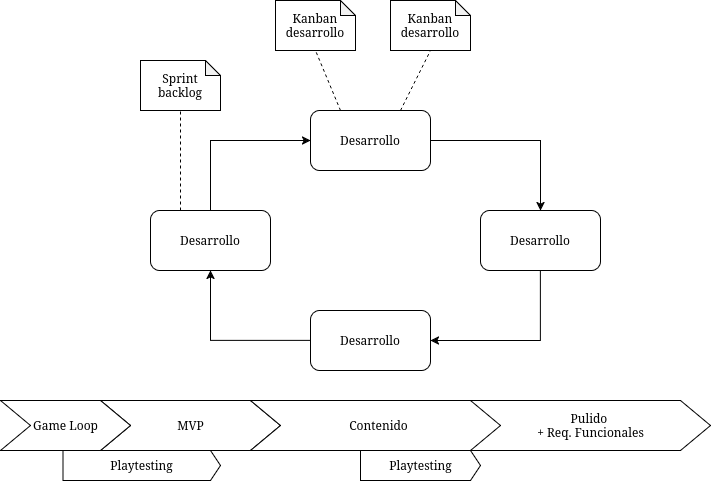
\includegraphics[scale=0.50]{img/updated-production.drawio.png}
    \caption[Diagrama de fase de producción revisada]{Diagrama revisado de la fase de producción.}
    \label{fig:updated-production}
\end{figure}